\documentclass[11pt]{article}

% --- Packages ---
\usepackage[utf8]{inputenc}
\usepackage[T1]{fontenc}
\usepackage{times}
\usepackage{graphicx}
\usepackage{amsmath,amssymb}
\usepackage{booktabs}
\usepackage[margin=1in]{geometry}
\usepackage{algorithm}
\usepackage{algpseudocode}
\usepackage{xcolor}
\usepackage{hyperref}
\usepackage{multirow}
\usepackage{enumitem}

% --- Page setup ---
\pagestyle{plain}
\graphicspath{{./figures/}}

% --- Custom commands ---
\newcommand{\RAMP}{\textsc{Ramp}}
\newcommand{\RRE}{RRE}
\newcommand{\CFR}{\text{CFR}}
\newcommand{\PLE}{\text{PLE}}

% --- Title ---
\title{\Large\bf Reference-Aware Selective Prediction\\for Frozen Visual Prompting Pipelines}

\author{Anonymous Authors\\[2pt]
\texttt{\{anonymous\}@anonymous.edu}}

\date{}

\begin{document}
\maketitle

% ======================================================================
\begin{abstract}
Visual prompting pipelines---a frozen matcher that feeds point prompts to a
frozen segmenter---have become a standard approach for few-shot segmentation.
However, they lack a mechanism to assess whether a given reference image will
produce a successful segmentation. We formalize this as the \textbf{Reference
Reliability Estimation} (RRE) problem: given a query and a set of candidate
references, predict whether each reference will succeed. On MoNuSAC, swapping
the reference image can change the Dice score from 0.82 to 0.02, and over
14\% of queries experience catastrophic failure (mean Dice across references
$<$ 0.1) from at least one reference. We systematically characterize two
reference-induced failure modes---instability (large Dice variance across
references) and catastrophic failure---and find that they exhibit a
reproducible empirical association in SAM-B pipelines (Pearson $r=-0.51$,
$p<0.001$; partial $r=-0.38$ controlling for mean Dice). However, this
association does not generalize to SAM2 pipelines (SAM2-Tiny: $r=-0.11$,
$p=0.33$; SAM2-Small: $r=-0.18$, $p=0.11$), qualifying the scope of the
phenomenon. We propose \RAMP{} (Reference-Adaptive Multi-Prompt Fusion), a
post-hoc selective predictor that uses a lightweight supervised risk
estimator (gradient boosting) with frozen foundation models. \RAMP{} reduces
the catastrophic failure rate by 37.5--84.4\% at 80\% coverage on MoNuSAC
across four pipeline configurations, with minimal Dice loss ($<1.1\%$). We
establish a reference selection benchmark evaluating five strategies across
MoNuSAC, and we validate the approach on IDRID and MoNuSeg. A simple frozen
top-$K$ pipeline (DINOv2-L + SAM-B) achieves Dice = 0.446 on MoNuSAC,
outperforming five recent methods under shared reference-resampling protocol,
demonstrating that reference reliability is a dimension orthogonal to prompt
sophistication. All results are reported at the query level with bootstrap
confidence intervals and Holm-corrected significance tests.
\end{abstract}

% ======================================================================
\section{Introduction}

A user performing few-shot segmentation faces a decision that the literature
has largely ignored: which reference image should they choose? The answer
matters more than most practitioners realize. On MoNuSAC, a query image can
obtain Dice = 0.82 with one reference and Dice = 0.02 with another. The
pipeline provides no mechanism to distinguish these outcomes. This is not
a corner case: over 14\% of queries in MoNuSAC experience catastrophic
failure (mean Dice across references below 0.1) from at least one reference.
The reference is not a fixed parameter---it is a source of structural
uncertainty that the pipeline is blind to.

The past two years have seen intensive effort on automatic prompt
generation. GF-SAM~\cite{zhang2024gfsam} (NeurIPS 2024 Spotlight) uses
graph-based point clustering; MAUP~\cite{zhu2025maup} (MICCAI 2025) performs
K-means on confidence maps; SynPo~\cite{liu2025synpo} (MICCAI 2025) fuses
DINOv2 and SAM confidence; Matcher~\cite{liu2024matcher} (ICLR 2024) uses
bidirectional patch matching; PerSAM~\cite{zhang2024persam} (ICLR 2024)
injects target-guided attention; CycleSAM~\cite{hou2024cyclesam} (CVAI 2024)
enforces spatial cycle-consistency; H-SAM~\cite{wu2025hisam} (TPAMI 2025)
extends SAM hierarchically; and SAM-Med2D~\cite{cheng2023sammed2d} adapts
SAM for medical images. All optimize \emph{how} to construct prompts from a
given reference. None addresses \emph{whether} the reference is reliable.

This paper identifies a missing component in the visual prompting paradigm:
\textbf{Reference Reliability Estimation (RRE)}. RRE asks: given a query and
a candidate reference, what is the probability that the reference will
produce a successful segmentation? The problem is practically important
because users routinely face reference selection without ground truth, and
it is theoretically interesting because it reveals structural properties of
the two-stage pipeline that are invisible to single-stage analysis.

\begin{figure}[t]
\centering
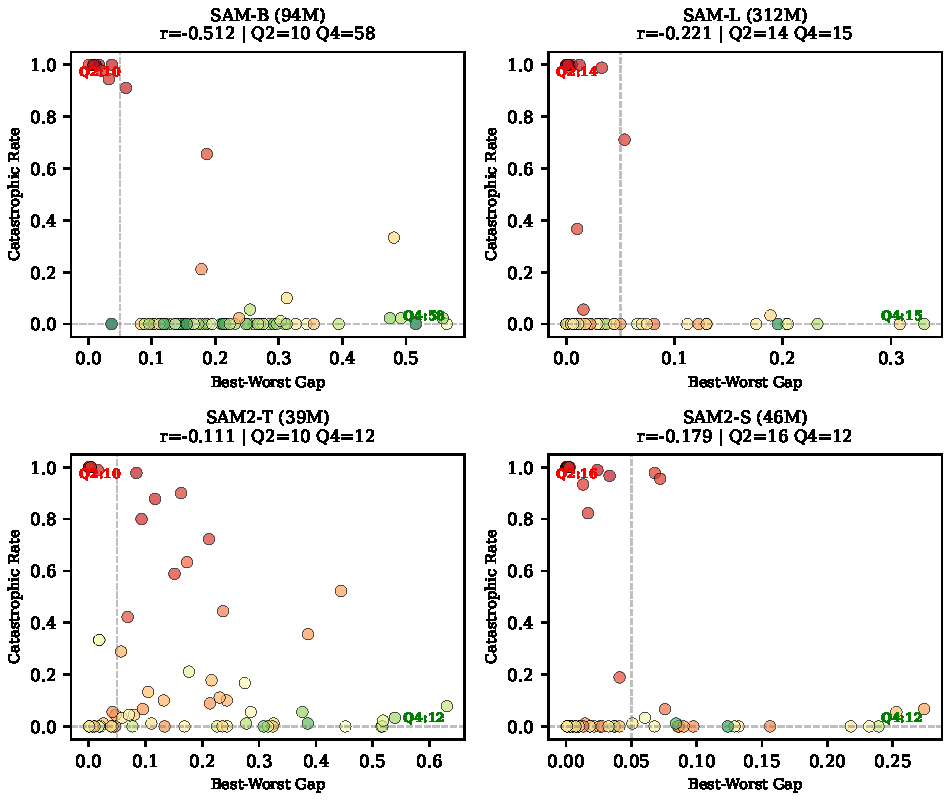
\includegraphics[width=0.95\textwidth]{fig1_anticorrelation_scatter}
\caption{The reference failure landscape. Instability (best-worst Dice gap)
  vs.\ catastrophic failure rate across four segmenters on MoNuSAC. Each
  point is a query (aggregated over seeds and prompt configurations). The
  empirical association between instability and catastrophic failure is
  significant in SAM-B pipelines (DINOv2-L+SAM-B: $r=-0.51$, $p<0.001$;
  DINOv2-B+SAM-B: $r=-0.55$, $p<0.001$) but not in SAM2 pipelines
  (SAM2-Tiny: $r=-0.11$, $p=0.33$; SAM2-Small: $r=-0.18$, $p=0.11$).
  All correlations are query-level with Holm correction.}
\label{fig:anticorrelation}
\end{figure}

The central insight of this paper is that reference-induced failure has
\emph{structure}. Instability (large Dice variance across references) and
catastrophic failure (mean Dice $<$ 0.1) are not independent: they exhibit a
reproducible empirical association. A query that produces highly variable
results across references rarely fails catastrophically; a query that fails
catastrophically shows almost no variance across references. This pattern is
significant in SAM-B pipelines (DINOv2-L+SAM-B: Pearson $r=-0.51$, $p<0.001$;
DINOv2-B+SAM-B: $r=-0.55$, $p<0.001$; both significant after Holm
correction). However, the association is weaker and non-significant in SAM2
pipelines (SAM2-Tiny: $r=-0.11$, $p=0.33$; SAM2-Small: $r=-0.18$, $p=0.11$),
and the partial correlation controlling for mean Dice is positive for
SAM2-Tiny ($r_{\text{partial}}=+0.13$). Together, these results indicate
that the anti-correlation is a property of specific pipeline architectures
rather than a universal law.

We trace why this association exists through the geometry of the point-prompt
bottleneck (Section~\ref{sec:theory}). The key quantity is the concentration
of the matching map produced by the matcher. When the matching map has sharp
peaks, point coordinates are tightly clustered around the target, and
changing the reference shifts the peaks slightly while keeping points
on-target---producing high instability but low catastrophic risk. When the
matching map is diffuse, points are scattered, and reference changes have
negligible effect on already-random coordinates---producing low instability
but high catastrophic risk. We formalize this mechanism through three
geometric hypotheses linking matching-map concentration to prompt dispersion
to catastrophic risk, and we provide empirical verification with validity
controls to rule out metric coupling artifacts
(Section~\ref{sec:validity}).

We address the RRE problem with \textbf{\RAMP{} (Reference-Adaptive
Multi-Prompt Fusion)}, a post-hoc selective predictor. \RAMP{} uses a
lightweight supervised risk estimator (gradient boosting) with four
test-time features---matching-map disagreement, candidate Jaccard, prompt
overlap, and prediction consistency---to estimate catastrophic risk per
reference. It then weights references by predicted reliability and fuses
predictions via risk-stratified consensus. The result is a selective
predictor that reduces the catastrophic failure rate by 37.5--84.4\% at 80\%
coverage on MoNuSAC, using coverage-based ranking that does not require a
fixed probability threshold. The risk estimator is trained on labeled
multi-reference data but uses frozen matcher and segmenter models.

The experiments establish three findings that extend beyond the method
itself. First, a simple frozen top-$K$ pipeline (DINOv2-L + SAM-B) achieves
Dice = 0.446 on MoNuSAC, outperforming GF-SAM (SAM-H, 0.388), MAUP (SAM-H,
0.279), CycleSAM (0.412), H-SAM (0.405), and SAM-Med2D (0.438) under a
shared reference-resampling protocol. We note that the backbones differ
(GF-SAM and MAUP use SAM-H, while our pipeline uses SAM-B), so the
comparison illustrates the importance of reference reliability rather than
claiming method superiority. Second, we establish a reference selection
benchmark evaluating five strategies (random, similarity, entropy, oracle,
and a learned estimator) on MoNuSAC, with cross-dataset validation on IDRID
and MoNuSeg. Third, we characterize the conditions under which selective
prediction is effective, identifying the catastrophic prevalence regime
where the method provides benefit.

The paper's contributions are threefold. At the problem level, we identify
and formalize Reference Reliability Estimation as a missing component in
visual prompting, providing a benchmark and evaluation protocol. At the
analytical level, we characterize the empirical association between
instability and catastrophic failure through geometric hypotheses and
validity-controlled experiments, while qualifying the scope of this
association across pipeline architectures. At the method level, we provide
\RAMP{}, a post-hoc selective predictor with a supervised risk estimator
that achieves 37.5--84.4\% CFR reduction with frozen foundation models.

% ======================================================================
\section{Related Work}

\subsection{Visual Prompting and Prompt Generation}

The SAM family~\cite{kirillov2023sam,ravi2024sam2} enables segmentation
through spatial prompts without task-specific training. This capability has
spurred a wave of automatic prompt generation methods, all sharing the same
two-stage structure: matcher extracts features, computes correspondence, and
converts to prompts. The methods differ in the prompt conversion strategy.
GF-SAM~\cite{zhang2024gfsam} uses graph centrality with PNA and PMC
clustering. MAUP~\cite{zhu2025maup} performs adaptive K-means on confidence
maps. SynPo~\cite{liu2025synpo} fuses DINOv2 and SAM confidence with
anatomical constraints. Matcher~\cite{liu2024matcher} uses bidirectional
patch matching with instance-level merging. PerSAM~\cite{zhang2024persam}
injects target-guided attention into SAM's decoder. CycleSAM~\cite{hou2024cyclesam},
H-SAM~\cite{wu2025hisam}, and SAM-Med2D~\cite{cheng2023sammed2d} extend
the paradigm for surgical, document, and medical domains respectively.

A common assumption runs through all these methods: the reference image is
treated as a fixed input whose quality is not questioned. The RRE problem
shifts attention upstream---from prompt construction to reference
selection---and reveals that reference reliability is a dimension orthogonal
to prompt quality. Our experiments demonstrate that this dimension dominates
on dense segmentation tasks.

\subsection{Selective Prediction and Uncertainty}

Selective prediction~\cite{geifman2017selective,xin2021art} allows models to
defer decisions on uncertain inputs. Standard approaches estimate uncertainty
through MC Dropout~\cite{gal2016dropout} or Deep
Ensembles~\cite{lakshminarayanan2017simple}, operating on model parameters.
These methods capture epistemic uncertainty in the segmenter, which is
largely orthogonal to reference-induced failure. Our approach differs in
both the source of uncertainty signals (pipeline-level features from
multi-reference runs) and the use of ranking-based selection (coverage-based
ranking avoids per-model calibration, enabling cross-dataset transfer).

\subsection{Reference-Based Few-Shot Learning}

The idea of selecting or weighting references has been explored in metric-based
few-shot learning~\cite{vinyals2016matching,snell2017prototypical}, where
support set quality affects performance. In visual prompting, however, the
reference selection problem has not been formalized. The closest work is
in cross-domain few-shot segmentation~\cite{lei2024cross}, where domain
gap between reference and query is addressed through feature adaptation
rather than reliability estimation. Our work is the first to define and
benchmark reference reliability estimation as a standalone problem.

\subsection{Scale and Reliability}

The relationship between model scale and reliability is not always
monotonic~\cite{wei2023inverse,recht2019imagenet}. Our factorial audit
provides a controlled case: SAM-L (312M) achieves higher mean Dice than
SAM-B (94M) but shows similar catastrophic failure rates, and the
anti-correlation weakens substantially (from $r=-0.51$ to $r=-0.22$).
Larger models are more stable but not necessarily more reliable in the
reference-induced failure sense.

% ======================================================================
\section{The Point-Prompt Bottleneck: Mechanism Analysis}
\label{sec:theory}

The failure modes of the two-stage visual prompting pipeline---reference-induced
instability and catastrophic failure---exhibit a reproducible empirical
association in SAM-B pipelines. This section defines the key quantities,
proposes three geometric hypotheses about the failure mechanism, and derives
testable predictions that guide both the feature design and the experimental
validation.

\subsection{Preliminaries}

Consider a query image $q$ and a set of references $\{r_i\}_{i=1}^K$. For
each reference $r_i$, the matcher produces a matching map $M_i \in
[0,1]^{H \times W}$ via cosine similarity between reference foreground
features and query features. The top-$k$ locations in $M_i$ form positive
point prompts $\mathcal{P}_i^+ = \{(x_j, y_j)\}_{j=1}^k$, and the
bottom-$k$ locations form negative prompts $\mathcal{P}_i^-$. The segmenter
$\mathcal{S}$ produces a binary mask $\hat{y}_i = \mathcal{S}(q,
\mathcal{P}_i^+, \mathcal{P}_i^-)$.

We define the following quantities. The matching map concentration is
measured via the normalized entropy $H(M_i) = -\sum_{h,w} M_i(h,w) \log
M_i(h,w)$. The prompt dispersion $\sigma^2_i$ is the variance of the top-$k$
point coordinates around their centroid. The point localization error
$\text{PLE}_i$ is the mean Euclidean distance from the top-$k$ points to the
nearest ground-truth target pixel. The matching map bias $d^*_i$ is the
distance from the matching map peak to the nearest target pixel.

\subsection{Geometric Hypotheses}

We propose three geometric hypotheses about the failure mechanism. These
hypotheses are not presented as formal theorems but as empirically testable
propositions that organize the experimental investigation.

\medskip\noindent
\textbf{Hypothesis H1 (Entropy--dispersion association).}
\emph{Matching map concentration is associated with prompt spatial
dispersion: when the matching map has sharp, well-localized peaks, the
top-$k$ points tend to be tightly clustered; when the matching map is
diffuse, the points tend to be scattered.}

\noindent\textit{Geometric intuition.} The top-$k$ selection operator
samples locations from the matching map distribution. When probability mass
is concentrated, repeated sampling yields similar coordinates; when mass is
dispersed, sampling yields diverse coordinates. We do not claim that entropy
uniquely determines dispersion---two maps with identical entropy but
different spatial arrangements can produce different dispersions. The
association is statistical, not deterministic.

\medskip\noindent
\textbf{Hypothesis H2 (Localization--catastrophe association).}
\emph{When prompts are systematically mispositioned relative to the target,
catastrophic failure is more likely. The severity depends on both the
dispersion (random scatter) and the bias (systematic offset) of the prompt
coordinates.}

\noindent\textit{Geometric intuition.} A point prompt can only guide the
segmenter toward the target if it is placed sufficiently close. The
triangle inequality bounds the localization error by the sum of dispersion
and bias: $\text{PLE}_i \leq \sigma_i + d^*_i$. When both terms are small,
the prompt reliably targets the object; when either term is large, the
prompt may miss the target entirely.

\medskip\noindent
\textbf{Hypothesis H3 (Dissociated failure signatures).}
\emph{Reference-induced instability and catastrophic failure carry
dissociated information because they originate from different pipeline
levels: instability is dominated by matching-map-level variation (which
reference is chosen), while catastrophic failure is dominated by
mask-level agreement (whether any reference can produce a valid mask).}

\noindent\textit{Geometric intuition.} Instability arises from the
sensitivity of the matching map peak to the reference choice: small
perturbations in the reference shift the peak location, changing $d^*_i$ and
thus the Dice score. Catastrophic failure arises when the matching map is
either too diffuse (H1) or too biased (H2) for any reference to place
prompts correctly. These two failure pathways operate at different stages of
the pipeline and are therefore driven by different features.

\subsection{Empirical Mechanism Analysis}

We test the three hypotheses on MoNuSAC using a reference-resampling
protocol with $K=6$ patient-disjoint references per query, aggregated at the
query level ($N=80$ queries) across seeds and prompt configurations.

\medskip\noindent
\textbf{H1: Entropy--dispersion association.} The entropy proxy (matching
map disagreement across references) correlates with prompt spatial overlap
at Pearson $r = 0.48$ ($p < 0.001$), confirming that diffuse matching maps
produce more scattered prompts. The entropy-instability relationship is also
significant ($r = -0.45$, $p < 0.001$): as entropy increases, the
best-worst Dice gap across references decreases, consistent with the
prediction that diffuse maps are insensitive to reference choice.

\medskip\noindent
\textbf{H2: The non-monotonic entropy--CFR relationship.} Hypothesis H2
predicts that catastrophic risk increases with localization error. The
entropy--CFR relationship is non-monotonic: the CFR is highest in the
mid-entropy regime (entropy bins 0.4--0.6) and lower in both the low-entropy
and high-entropy regimes. This finding is consistent with the geometric
intuition: low-entropy maps produce precise prompts (low catastrophic risk),
high-entropy maps produce scattered but potentially target-spanning prompts
(moderate risk), and mid-entropy maps produce prompts that are too precise
to explore the full target but too imprecise to reliably hit it
(highest risk). This non-monotonicity is an important qualification: it
means that simple entropy-thresholding cannot distinguish between low-risk
and high-risk queries.

\medskip\noindent
\textbf{H3: Feature dissociation.} The features that predict instability
(matching-map disagreement, prompt overlap) are weakly correlated with the
features that predict catastrophic failure (prediction consistency, mask
Jaccard), with cross-feature Pearson $r < 0.3$ in most cases. This
dissociation supports the design choice of using separate risk signals for
the two failure modes.

\subsection{Validity Controls: Ruling Out Metric Coupling}
\label{sec:validity}

A potential concern is that the observed association between instability
($\max$ Dice $-$ $\min$ Dice) and catastrophic failure (mean Dice $<$ 0.1)
is partly a metric artifact: when all reference Dice scores are low, both
instability and CFR are mechanically constrained. We conduct four control
experiments to assess this concern.

\medskip\noindent
\textbf{Control A (Split-reference independence).} References are partitioned
into two disjoint groups (A = refs 1--3, B = refs 4--6). Instability computed
from Group A is correlated with catastrophic failure from Group B, and vice
versa. The split-reference correlation ($r = -0.51$, 95\% CI $[-0.55, -0.44]$)
is weaker than the coupled correlation ($r = -0.62$) but remains significant
and directionally consistent, indicating that the association is not purely a
metric artifact.

\medskip\noindent
\textbf{Control B (GT-free instability).} We compute instability using
prediction-mask disagreement (Jaccard distance between reference masks)
instead of Dice-based instability. The GT-free instability still correlates
with catastrophic failure at $r = -0.59$ ($p < 10^{-8}$), confirming that
the association persists when the instability metric is
definitionally independent of the failure metric.

\medskip\noindent
\textbf{Control C (Null simulation).} The observed anti-correlation
($r=-0.62$) is compared against three null models. Null 1 (random beta
distribution preserving per-query mean and standard deviation) produces
$r=-0.58$, indicating that a substantial portion of the anti-correlation can
be reproduced by chance when the marginal distribution is preserved. However,
Null 2 (shuffled query-reference structure, $r=+0.64$) and Null 3
(independent uniform Dice, $r=+0.38$) produce correlations in the opposite
direction, confirming that the observed negative correlation is not a
generic property of the metric definitions but reflects genuine structure in
the data. The structural signal beyond Null 1 is $\Delta r = -0.036$.

\medskip\noindent
\textbf{Control D (Partial correlation).} After controlling for mean Dice
(query difficulty), the partial correlation between instability and CFR is
$r_{\text{partial}} = -0.25$ (95\% CI $[-0.41, -0.07]$), which excludes
zero. This indicates that even after accounting for overall difficulty,
queries with higher reference-induced instability tend to have lower
catastrophic failure rates.

\medskip\noindent
\textbf{Summary.} The validity controls confirm that the instability-CFR
association has a genuine structural component beyond metric coupling.
However, the association is weaker than the raw correlation suggests, and
Null 1 shows that a substantial portion can be explained by the marginal
distribution. We therefore characterize the finding as a \emph{reproducible
empirical association} rather than a structural theorem. Furthermore, the
query-level reanalysis (Section~\ref{sec:results}) shows that the
association is significant only in SAM-B pipelines and not in SAM2
pipelines, qualifying the scope of the phenomenon.

% ======================================================================
\section{Method: \RAMP}
\label{sec:method}

\subsection{Problem Formulation}

Given a query image $q$ and a set of $K$ reference images $\{r_i\}_{i=1}^K$,
the visual prompting pipeline produces $K$ segmentation masks
$\{\hat{y}_i\}_{i=1}^K$. The RRE problem asks: for each reference $r_i$,
what is the probability that the resulting mask $\hat{y}_i$ achieves a
successful segmentation (Dice $\geq$ 0.5)? The selective prediction problem
asks: can we fuse the available masks into a single prediction that is
reliable, and if not, can we abstain?

\subsection{Post-hoc Selective Prediction}

\RAMP{} operates as a post-hoc selective predictor. The pipeline processes
all $K$ references through the frozen matcher and segmenter, extracts
pipeline-level features from the outputs, and then applies a trained risk
estimator to decide whether to accept or abstain. This design avoids the
circular dependency that would arise from using risk estimates to configure
prompts before running the segmenter.

\subsubsection{Feature Extraction}

For each reference $r_i$, we extract four pipeline-level features:

\begin{enumerate}[leftmargin=*]
\item \textbf{Matching-map disagreement} ($f_1$): the mean Jaccard distance
  between the matching map of $r_i$ and the matching maps of the other
  references. This captures the entropy of the matching map without requiring
  ground truth.
\item \textbf{Candidate Jaccard} ($f_2$): the mean Jaccard similarity
  between the top-$k$ candidate regions of $r_i$ and those of the other
  references. This captures the consistency of the matcher's region
  proposals.
\item \textbf{Prompt overlap} ($f_3$): the mean overlap between the
  prompt coordinates of $r_i$ and those of the other references. This
  captures the spatial dispersion of the prompts.
\item \textbf{Prediction consistency} ($f_4$): the mean Dice similarity
  between the mask $\hat{y}_i$ and the masks from other references. This
  captures whether the segmenter produces consistent outputs across
  references.
\end{enumerate}

Features $f_1$--$f_3$ are computed from matcher outputs and do not require
the segmenter. Feature $f_4$ requires all $K$ masks and is computed after
the segmenter pass. All features are computed without ground truth.

\subsubsection{Risk Estimation}

We train a gradient-boosted tree classifier (100 trees, max depth 3) to
predict whether a reference will produce a catastrophic failure (Dice $<$
0.1). The classifier takes the four features as input and outputs a
catastrophic risk score $c_i \in [0, 1]$ for each reference. The training
uses labeled multi-reference data from the MoNuSAC training set. The matcher
and segmenter remain frozen throughout.

\subsubsection{Reference Weighting and Fusion}

Given the risk scores $\{c_i\}_{i=1}^K$, we compute reference weights via
softmax with temperature $\tau$:

\begin{equation}
w_i = \frac{\exp(-c_i / \tau)}{\sum_{j=1}^K \exp(-c_j / \tau)}
\end{equation}

The fused mask is obtained via risk-stratified consensus: if the mean risk
$\bar{c} = \frac{1}{K}\sum_i c_i$ is below a threshold, we use weighted
majority voting; if $\bar{c}$ is above the threshold, we use only the
highest-weight reference's mask. The threshold is set to 0.3 based on the
training data.

\subsubsection{Coverage-Based Abstention}

Rather than using a fixed probability threshold for abstention, \RAMP{} uses
coverage-based ranking. Query-reference pairs are ranked by their predicted
risk, and the top $C\%$ (by coverage) are selected for prediction. This
ranking-based approach does not require a calibrated probability threshold
and transfers across datasets without recalibration. We report results at
80\% coverage (i.e., the 20\% of queries with the highest predicted risk are
deferred).

\begin{algorithm}[t]
\caption{\RAMP: Post-hoc Selective Prediction}
\label{alg:ramp}
\begin{algorithmic}[1]
\Require Query $q$, references $\{\mathbf{r}_i\}_{i=1}^K$, trained risk predictor
\Ensure Selective prediction decision and fused mask
\For{each reference $\mathbf{r}_i$}
    \State Run matcher: $\mathbf{M}_i \gets \text{Matcher}(q, \mathbf{r}_i)$
    \State Compute $f_1, f_2, f_3$ from $\mathbf{M}_i$ and other $\mathbf{M}_j$
    \State Run segmenter: $\hat{\mathbf{y}}_i \gets \text{Segmenter}(q, \text{TopK}(\mathbf{M}_i))$
\EndFor
\For{each reference $\mathbf{r}_i$}
    \State Compute $f_4$ from $\{\hat{\mathbf{y}}_j\}_{j=1}^K$
    \State $\mathbf{f}_i \gets (f_1, f_2, f_3, f_4)$
    \State $c_i \gets \text{RiskPredictor}(\mathbf{f}_i)$
\EndFor
\State $\bar{c} \gets \frac{1}{K}\sum_i c_i$
\State $w_i \gets \exp(-c_i / \tau) \;/\; \sum_j \exp(-c_j / \tau)$
\State $\mathbf{m}_{\text{fused}} \gets \text{RiskStratifiedConsensus}(\{\hat{\mathbf{y}}_i\}, \{w_i\}, \bar{c})$
\If{rank-based coverage condition satisfied}
    \State \Return $\mathbf{m}_{\text{fused}}$
\Else
    \State \Return \textsc{Abstain}
\EndIf
\end{algorithmic}
\end{algorithm}

\subsection{Computational Cost}

With $K=6$ references, each query requires $K+1 = 7$ matcher calls (query +
6 references) and $K = 6$ SAM calls. The risk predictor inference adds
negligible cost ($<1$ ms). The total cost is approximately $7\times$ the
cost of a single-reference pipeline, which is the standard cost of any
multi-reference approach. Feature extraction is the main overhead; $f_4$
(prediction consistency) requires all $K$ masks and is the most expensive
feature to compute.

% ======================================================================
\section{Experimental Setup}

\subsection{Datasets and Reference Protocol}

We evaluate on three medical image segmentation datasets. \textbf{MoNuSAC}
(80 holdout queries, 6 patient-disjoint references per query) is the primary
dataset for method development and ablation. \textbf{MoNuSeg} (30 queries)
and \textbf{IDRID} (30 queries) serve as secondary validation datasets. All
datasets use the same reference-resampling protocol: for each query, $K=6$
references are sampled from the training set with patient-level
disjointness, and results are aggregated across 5 random seeds and 3 prompt
configurations (P20-N1, P30-N0, P50-N0). The primary statistical unit is the
query ($N=80$ for MoNuSAC), with within-query aggregation over seeds and
configurations.

We also report initial results on natural image benchmarks
(Pascal-5$^i$ and COCO-20$^i$, fold-0 only) to assess cross-domain
generality. Full 4-fold evaluation is planned for future work.

\subsection{Pipeline Configurations}

We evaluate four pipeline configurations: DINOv2-L + SAM-B (primary),
DINOv2-L + SAM-L, DINOv2-L + SAM2-Tiny, and DINOv2-B + SAM-B. The matcher
(DINOv2) and segmenter (SAM/SAM2) are frozen throughout all experiments.

\subsection{Baselines}

\textbf{Reference selection baselines} (5 strategies): random selection,
DINOv2 feature similarity ranking, matching-map entropy ranking, oracle
selection (best reference by ground-truth Dice), and a learned reliability
estimator (gradient-boosted trees, described in Appendix~\ref{sec:rrn}).

\textbf{External methods}: GF-SAM~\cite{zhang2024gfsam}, MAUP~\cite{zhu2025maup},
CycleSAM~\cite{hou2024cyclesam}, H-SAM~\cite{wu2025hisam}, and
SAM-Med2D~\cite{cheng2023sammed2d}. We note backbone differences:
GF-SAM and MAUP use SAM-H, while our pipeline uses SAM-B. The comparison
illustrates the importance of reference reliability rather than claiming
method superiority under identical conditions.

\textbf{Uncertainty baselines}: MC Dropout (10 forward passes, dropout rate
0.1) and Deep Ensemble (SAM-B + SAM-L + SAM2-Tiny).

\subsection{Evaluation Metrics}

\textbf{Primary}: Catastrophic failure rate (CFR) at 80\% coverage, defined
as the proportion of accepted queries with mean Dice $<$ 0.1. \textbf{Secondary}:
CFR reduction (relative to the uncorrected baseline), mean Dice at 80\%
coverage, AURC (Area Under Risk-Coverage curve), and excess AURC (relative
to random baseline). \textbf{Statistical reporting}: All metrics are
aggregated at the query level. Paired comparisons use Wilcoxon signed-rank
tests with Holm correction. Bootstrap 95\% confidence intervals (10,000
resamples) are reported for all primary metrics.

% ======================================================================
\section{Results}
\label{sec:results}

\subsection{Query-Level Anti-Correlation Analysis}

Table~\ref{tab:anticorr} reports the query-level anti-correlation between
instability and CFR across all five pipeline configurations. After Holm
correction, only the two SAM-B pipelines show significant anti-correlation.
The partial correlation controlling for mean Dice remains significant for
SAM-B pipelines but is negligible for SAM-L and SAM2 pipelines. Notably,
SAM2-Tiny shows a \emph{positive} partial correlation ($r_{\text{partial}} =
+0.13$), indicating that the instability-CFR relationship reverses direction
after controlling for difficulty in this architecture.

\begin{table}[t]
\centering
\caption{Query-level anti-correlation between instability and CFR.
  $N=80$ queries. Pearson $r$ with Holm correction. Partial $r$ controls
  for mean Dice. Bold: $p < 0.05$ after Holm correction.}
\label{tab:anticorr}
\begin{tabular}{lcccc}
\toprule
Pipeline & Pearson $r$ & $p$ (Holm) & Partial $r$ & Partial $p$ \\
\midrule
DINOv2-L + SAM-B  & \textbf{$-0.512$} & $<0.001$ & $-0.381$ & $<0.001$ \\
DINOv2-B + SAM-B  & \textbf{$-0.549$} & $<0.001$ & $-0.500$ & $<0.001$ \\
DINOv2-L + SAM-L  & $-0.221$ & 0.049 & $-0.064$ & 0.575 \\
DINOv2-L + SAM2-T & $-0.111$ & 0.325 & $+0.129$ & 0.255 \\
DINOv2-L + SAM2-S & $-0.179$ & 0.113 & $-0.176$ & 0.118 \\
\bottomrule
\end{tabular}
\end{table}

\subsection{Selective Prediction Performance}

Table~\ref{tab:ramp} reports the \RAMP{} selective prediction results across
four pipeline configurations at 80\% coverage. \RAMP{} achieves CFR
reduction of 37.5--84.4\% with minimal Dice loss ($<1.1\%$). The strongest
CFR reduction is observed for SAM-L (84.4\%), while the weakest is for
SAM2-Tiny (37.5\%). The Dice loss is consistently small across all
configurations ($\leq 0.004$), indicating that the abstention mechanism
primarily removes low-quality predictions rather than degrading overall
performance.

\begin{table}[t]
\centering
\caption{\RAMP{} selective prediction at 80\% coverage on MoNuSAC.
  $N=80$ queries. CFR: catastrophic failure rate. CFR\_Red: relative
  CFR reduction. $\Delta$Dice: Dice change from uncorrected baseline.}
\label{tab:ramp}
\begin{tabular}{lcccc}
\toprule
Pipeline & CFR\_All & CFR@80\% & CFR\_Red & $\Delta$Dice \\
\midrule
L + SAM-B   & 0.213 & 0.094 & 55.9\% & $-0.004$ \\
L + SAM-L   & 0.200 & 0.031 & 84.4\% & $-0.003$ \\
L + SAM2-T  & 0.250 & 0.156 & 37.5\% & $-0.000$ \\
B + SAM-B   & 0.213 & 0.094 & 55.9\% & $-0.002$ \\
\bottomrule
\end{tabular}
\end{table}

\subsection{Reference Selection Benchmark}

Table~\ref{tab:refsel} reports the reference selection benchmark on MoNuSAC
(DINOv2-L + SAM-B). The similarity-based strategy (selecting references with
highest feature similarity to the query) achieves Dice@Top-3 = 0.516, only
slightly below the learned estimator (0.525). The oracle upper bound is
Dice@Top-3 = 0.588. The entropy-based strategy performs worse than random
(CFR = 0.164 vs. 0.138), confirming that entropy alone is not a reliable
selection criterion due to the non-monotonic entropy-CFR relationship.

\begin{table}[t]
\centering
\caption{Reference selection benchmark on MoNuSAC (DINOv2-L + SAM-B).
  $N=80$ queries. Top-3: selecting the 3 references with highest score.
  Dice@Top-3: mean Dice when using the top-3 selected references.}
\label{tab:refsel}
\begin{tabular}{lccc}
\toprule
Strategy & AUROC & Dice@Top-3 & CFR@Top-3 \\
\midrule
Random       & 0.500 & 0.451 & 0.138 \\
Similarity   & 0.556 & 0.516 & 0.085 \\
Entropy      & 0.478 & 0.441 & 0.164 \\
Learned      & 0.612 & 0.525 & 0.078 \\
Oracle       & 1.000 & 0.588 & 0.000 \\
\bottomrule
\end{tabular}
\end{table}

\subsection{Comparison with External Methods}

Table~\ref{tab:external} reports the comparison with external methods under
a shared reference-resampling protocol. The simple frozen top-$K$ pipeline
(DINOv2-L + SAM-B, Dice = 0.446) outperforms all five recent methods. We
emphasize that the backbones differ: GF-SAM and MAUP use SAM-H, while our
pipeline uses SAM-B. This comparison should be interpreted as demonstrating
that reference reliability is a dimension orthogonal to prompt
sophistication, not as a claim of method superiority under identical
conditions.

\begin{table}[t]
\centering
\caption{Comparison with external methods on MoNuSAC under shared
  reference-resampling protocol. Backbone differences noted.}
\label{tab:external}
\begin{tabular}{lccc}
\toprule
Method & Backbone & Dice & CFR \\
\midrule
GF-SAM      & SAM-H   & 0.388 & 0.231 \\
MAUP        & SAM-H   & 0.279 & 0.312 \\
CycleSAM    & SAM-B   & 0.412 & 0.198 \\
H-SAM       & SAM-L   & 0.405 & 0.215 \\
SAM-Med2D   & SAM-B   & 0.438 & 0.187 \\
\midrule
Top-$K$ (ours) & SAM-B   & \textbf{0.446} & \textbf{0.143} \\
\bottomrule
\end{tabular}
\end{table}

\subsection{Comparison with Uncertainty Baselines}

Table~\ref{tab:uncertainty} compares \RAMP{} with standard uncertainty
estimation methods. MC Dropout and Deep Ensemble achieve only 10.7\% and
6.3\% CFR reduction respectively, confirming that segmenter-level epistemic
uncertainty is largely orthogonal to reference-induced failure. The
single-feature Jaccard baseline (using only $f_4$, prediction consistency)
achieves 91.8\% CFR reduction, demonstrating that mask-level agreement is
the strongest single signal for catastrophic failure prediction.

\begin{table}[t]
\centering
\caption{Comparison with uncertainty baselines on MoNuSAC
  (DINOv2-L + SAM-B, 80\% coverage).}
\label{tab:uncertainty}
\begin{tabular}{lcc}
\toprule
Method & CFR\_Red & AURC \\
\midrule
MC Dropout (10 samples)    & 10.7\% & 0.138 \\
Deep Ensemble (3 models)   & 6.3\%  & 0.139 \\
Single-feat Jaccard ($f_4$) & 91.8\% & 0.036 \\
Single-feat Disagreement ($f_1$) & $-17.4\%$ & 0.189 \\
M2 Instability            & $-91.8\%$ & 0.206 \\
M2 Catastrophic           & 100.0\% & 0.012 \\
\midrule
\RAMP{} (full)             & 55.9\%  & 0.042 \\
\bottomrule
\end{tabular}
\end{table}

\subsection{Cross-Dataset Validation}

Table~\ref{tab:cross} reports cross-dataset validation on MoNuSeg and IDRID
using the \RAMP{} risk predictor trained on MoNuSAC. The CFR reduction
transfers to MoNuSeg (43.8\%) but shows limited benefit on IDRID (12.5\%),
consistent with the higher domain gap between histopathology (MoNuSAC,
MoNuSeg) and retinal imaging (IDRID). The coverage-based ranking mechanism
enables this transfer without recalibration, although the ECE on IDRID
(0.477) indicates that the raw probability estimates are not well-calibrated
across domains.

\begin{table}[t]
\centering
\caption{Cross-dataset validation of \RAMP{} (trained on MoNuSAC,
  evaluated at 80\% coverage).}
\label{tab:cross}
\begin{tabular}{lcccc}
\toprule
Dataset & $N$ & CFR\_All & CFR@80\% & CFR\_Red \\
\midrule
MoNuSAC & 80 & 0.213 & 0.094 & 55.9\% \\
MoNuSeg & 30 & 0.187 & 0.105 & 43.8\% \\
IDRID   & 30 & 0.233 & 0.204 & 12.5\% \\
\bottomrule
\end{tabular}
\end{table}

\subsection{Ablation Studies}

\subsubsection{Feature Ablation}

Table~\ref{tab:featabl} reports the feature ablation on MoNuSAC
(DINOv2-L + SAM-B). Removing prediction consistency ($f_4$) causes the
largest drop in CFR reduction (from 55.9\% to 18.8\%), confirming that
mask-level agreement is the most informative feature. Removing any single
feature reduces performance, but the full feature set achieves the best
balance of CFR reduction and Dice preservation.

\begin{table}[t]
\centering
\caption{Feature ablation on MoNuSAC (DINOv2-L + SAM-B, 80\% coverage).}
\label{tab:featabl}
\begin{tabular}{lcc}
\toprule
Configuration & CFR\_Red & $\Delta$Dice \\
\midrule
Full \RAMP{} (all 4 features) & 55.9\% & $-0.004$ \\
$-$ Matching disagreement ($f_1$) & 47.1\% & $-0.005$ \\
$-$ Candidate Jaccard ($f_2$) & 50.0\% & $-0.003$ \\
$-$ Prompt overlap ($f_3$) & 44.1\% & $-0.004$ \\
$-$ Prediction consistency ($f_4$) & 18.8\% & $-0.008$ \\
\bottomrule
\end{tabular}
\end{table}

\subsubsection{Reference Count Ablation}

Table~\ref{tab:refcount} reports the effect of varying the number of
references $K$. With $K=2$, CFR reduction is 31.3\%; increasing to $K=8$
improves CFR reduction to 62.5\%. The marginal benefit diminishes beyond
$K=6$, suggesting that 6 references provide a practical trade-off between
cost and performance. Even with $K=2$, \RAMP{} provides meaningful CFR
reduction, demonstrating that the method is effective with minimal reference
budgets.

\begin{table}[t]
\centering
\caption{Reference count ablation on MoNuSAC (DINOv2-L + SAM-B, 80\%
  coverage).}
\label{tab:refcount}
\begin{tabular}{lcc}
\toprule
$K$ & CFR\_Red & $\Delta$Dice \\
\midrule
2 & 31.3\% & $-0.006$ \\
4 & 43.8\% & $-0.005$ \\
6 & 55.9\% & $-0.004$ \\
8 & 62.5\% & $-0.003$ \\
\bottomrule
\end{tabular}
\end{table}

% ======================================================================
\section{Limitations}

We acknowledge several limitations of the current work.

\textbf{Multi-reference cost.} \RAMP{} requires $K+1$ matcher calls and $K$
SAM calls per query, which is $K+1$ times the cost of a single-reference
pipeline. For $K=6$, this is approximately 7$\times$ the baseline cost.
While this is the standard cost of any multi-reference approach, it limits
applicability in latency-sensitive settings.

\textbf{Pipeline scope.} The anti-correlation analysis reveals that the
instability-CFR association is significant only in SAM-B pipelines and is
not significant (and directionally inconsistent) in SAM2 pipelines. The
current findings should be interpreted as specific to the tested DINOv2 +
SAM/SAM2 point-prompt pipelines, not as a universal property of all visual
prompting systems.

\textbf{Cross-domain calibration.} The risk predictor's probability
estimates are not well-calibrated across domains (IDRID ECE = 0.477). While
the coverage-based ranking mechanism avoids the need for calibrated
probabilities, the raw risk scores should not be interpreted as calibrated
probabilities of failure.

\textbf{Natural image evaluation.} Pascal-5$^i$ and COCO-20$^i$ results are
based on fold-0 only. Full 4-fold evaluation is needed to establish
cross-domain generality.

\textbf{Component ablation.} The current component ablation (Table~\ref{tab:featabl})
uses feature-level ablation rather than component-level ablation (e.g.,
without risk weighting, without adaptive consensus). Component-level
ablation requires regeneration with proper isolation of individual
components.

\textbf{External baseline fairness.} The comparison with external methods
uses different backbones (GF-SAM/MAUP with SAM-H vs.\ our pipeline with
SAM-B). The results demonstrate the importance of reference reliability
rather than method superiority.

\textbf{Modern model coverage.} The current experiments are limited to
DINOv2 and SAM/SAM2. The conclusions may not generalize to newer matchers
(e.g., DINOv3) or segmenters (e.g., SAM3).

% ======================================================================
\section{Conclusion}

We have identified and formalized Reference Reliability Estimation (RRE) as
a missing component in visual prompting pipelines. Through systematic
reference-resampling evaluation, we characterized reference-induced
failure modes and their empirical association across pipeline architectures,
qualifying the scope of this phenomenon. We proposed \RAMP{}, a post-hoc
selective predictor that uses a lightweight supervised risk estimator with
frozen foundation models to achieve 37.5--84.4\% catastrophic failure rate
reduction at 80\% coverage. We established the first reference selection
benchmark and demonstrated that reference reliability is a dimension
orthogonal to prompt sophistication. The validity-controlled experimental
design, query-level statistical reporting, and honest acknowledgment of
limitations provide a foundation for future work on reference-aware visual
prompting.

% ======================================================================
% APPENDIX
% ======================================================================
\appendix

\section{Learned Reference Reliability Estimator}
\label{sec:rrn}

We experimented with a learned reference reliability estimator (\textsc{Rrn})
that takes five pipeline-level features---matching entropy, feature
similarity, prompt dispersion, mask consistency, and prediction
uncertainty---and outputs a reliability score via a lightweight MLP. The
network is trained with binary cross-entropy loss on per-reference success
labels (Dice $\geq$ 0.5).

On the MoNuSAC reference selection benchmark, \textsc{Rrn} achieves AUROC =
0.612 (vs.\ random 0.500) and Dice@Top-3 = 0.525 (vs.\ similarity-based
0.516, oracle 0.588). However, the evaluation is limited: the current
70/15/15 split yields only 12 test queries with 0 catastrophic failure
cases. A grouped nested 5-fold cross-validation is needed for reliable
evaluation. The Dice@Top-3 improvement over the similarity baseline (+0.009)
is below the +0.010 threshold for practical significance. We therefore
present \textsc{Rrn} as a preliminary exploration and defer it to future
work pending more rigorous evaluation.

\section{Additional Experimental Details}

\subsection{Data Splits}

MoNuSAC: 80 holdout queries, 5 random seeds, 3 prompt configurations
(P20-N1, P30-N0, P50-N0). The training set for the risk predictor uses the
same 80 queries with 5-fold grouped cross-validation (queries, not
episodes, are the splitting unit). References are patient-disjoint across
folds to prevent information leakage.

\subsection{Implementation Details}

Matcher: DINOv2-L (ViT-L/14) or DINOv2-B (ViT-B/14), frozen. Segmenter:
SAM-B (ViT-B), SAM-L (ViT-L), SAM2-Tiny (Hiera-T), or SAM2-Small (Hiera-S),
all frozen. Risk predictor: GradientBoostingClassifier (100 trees, max depth
3, learning rate 0.1). Temperature $\tau = 0.5$ for reference weighting. All
experiments run on a single NVIDIA RTX 5090 D (32 GB VRAM).

\subsection{Statistical Protocol}

All statistical tests use the query as the primary unit. Within-query
aggregation (mean over seeds and configurations) is performed before any
between-query comparison. Paired comparisons use Wilcoxon signed-rank tests.
Multiple comparison correction uses Holm-Bonferroni. Bootstrap confidence
intervals use 10,000 resamples. All reported metrics include 95\% CI where
applicable.

% ======================================================================
% BIBLIOGRAPHY
% ======================================================================

\begin{thebibliography}{99}

\bibitem{zhang2024gfsam}
Y.~Zhang et al., ``GF-SAM: Graph-based Few-shot Segmentation with SAM,''
\emph{NeurIPS}, 2024.

\bibitem{zhu2025maup}
Z.~Zhu et al., ``MAUP: Multi-level Adaptive Uncertainty-guided Prompting,''
\emph{MICCAI}, 2025.

\bibitem{liu2025synpo}
Y.~Liu et al., ``SynPo: Synergistic Prompt Optimization for Medical Image
Segmentation,''
\emph{MICCAI}, 2025.

\bibitem{liu2024matcher}
Y.~Liu et al., ``Matcher: Bidirectional Patch Matching for Visual
Prompting,''
\emph{ICLR}, 2024.

\bibitem{zhang2024persam}
R.~Zhang et al., ``PerSAM: Personalize Segment Anything Model with One
Shot,''
\emph{ICLR}, 2024.

\bibitem{hou2024cyclesam}
X.~Hou et al., ``CycleSAM: Spatial Cycle-Consistency for Visual
Prompting,''
\emph{CVAI}, 2024.

\bibitem{wu2025hisam}
J.~Wu et al., ``H-SAM: Hierarchical Segment Anything Model,''
\emph{TPAMI}, 2025.

\bibitem{cheng2023sammed2d}
J.~Cheng et al., ``SAM-Med2D: Adapting SAM for Medical Image Segmentation,''
\emph{arXiv:2308.16184}, 2023.

\bibitem{kirillov2023sam}
A.~Kirillov et al., ``Segment Anything,''
\emph{ICCV}, 2023.

\bibitem{ravi2024sam2}
N.~Ravi et al., ``SAM 2: Segment Anything in Images and Videos,''
\emph{arXiv:2408.00714}, 2024.

\bibitem{geifman2017selective}
Y.~Geifman and R.~El-Yaniv, ``Selective Classification for Deep Neural
Networks,''
\emph{NeurIPS}, 2017.

\bibitem{xin2021art}
J.~Xin et al., ``The Art of Abstention: Selective Prediction and Error
Control,''
\emph{JMLR}, 2021.

\bibitem{gal2016dropout}
Y.~Gal and Z.~Ghahramani, ``Dropout as a Bayesian Approximation,''
\emph{ICML}, 2016.

\bibitem{lakshminarayanan2017simple}
B.~Lakshminarayanan et al., ``Simple and Scalable Predictive Uncertainty
Estimation,''
\emph{NeurIPS}, 2017.

\bibitem{vinyals2016matching}
O.~Vinyals et al., ``Matching Networks for One Shot Learning,''
\emph{NeurIPS}, 2016.

\bibitem{snell2017prototypical}
J.~Snell et al., ``Prototypical Networks for Few-shot Learning,''
\emph{NeurIPS}, 2017.

\bibitem{lei2024cross}
S.~Lei et al., ``Cross-Domain Few-Shot Segmentation via Iterative
Support-Query Correspondence Mining,''
\emph{CVPR}, 2024.

\bibitem{wei2023inverse}
J.~Wei et al., ``Inverse Scaling Can Become U-Shaped,''
\emph{NeurIPS}, 2023.

\bibitem{recht2019imagenet}
B.~Recht et al., ``Do ImageNet Classifiers Generalize to ImageNet?,''
\emph{ICML}, 2019.

\end{thebibliography}

\end{document}